%%%%%%%%%%%%%%%%%%%%%%%%%%%%%%%%%%%%%%%%%%%%%%%%%%%%%%%%%%%%%%%
%
% Welcome to Overleaf --- just edit your LaTeX on the left,
% and we'll compile it for you on the right. If you open the
% 'Share' menu, you can invite other users to edit at the same
% time. See www.overleaf.com/learn for more info. Enjoy!
%
%%%%%%%%%%%%%%%%%%%%%%%%%%%%%%%%%%%%%%%%%%%%%%%%%%%%%%%%%%%%%%%
\documentclass{beamer}
\usepackage{color}
\usepackage{graphicx}

\setbeamertemplate{caption}{\raggedright\insertcaption\par}

\usetheme{Copenhagen}


%Information to be included in the title page:
\title{Metodi di ottimizzazione su varietà differenziabili per la media di Fréchet su disco di Poincaré}
\author{\texorpdfstring{Candidato: Luca Moroni \\Relatore: Bruno Iannazzo}{Candidato}}
\date{Anno Accademico 2020/2021}

\begin{document}

\frame{\titlepage}

\begin{frame}
\frametitle{Introduzione}
\begin{beamerboxesrounded}{}
Tratteremo \alert{metodi di ottimizzazione} di funzioni definite su \alert{varietà differenziabili}, oggetti geometrici che generalizzano le nozioni di curva e superficie a dimensioni maggiori.
\bigskip
\end{beamerboxesrounded}
\begin{center}
    \includegraphics[height=3.5cm]{manopt2.png} 
\end{center}
\end{frame}

\begin{frame}
\frametitle{Introduzione}
\begin{beamerboxesrounded}{Problema}
Calcolare il centroide di $p$ punti nel \textbf{disco di Poincaré}.
\end{beamerboxesrounded}
\bigskip
\begin{itemize}
    \item Radar clutter classification [Barbasesco et al., 2019] % Thales Francia, Leonardo Italia.
    \item Hyperbolic deep neural networks [Peng et al., 2021]
\end{itemize}
\bigskip
\begin{center}
    \includegraphics[height=3.5cm]{escher_disk.png} 
\end{center}
\end{frame}

\begin{frame}
\frametitle{Ottimizzazione euclidea}
Data $f : \mathbb{R}^n \to \mathbb{R}$, con $f$ due volte differenziabile, cercheremo di trovare un punto di minimo di $f$.
Condizioni necessarie per dire se x è un punto di minimo:\\~\

\begin{itemize}
\item $\nabla f(x) = 0$
\item $\nabla^2 f(x)$ definita positiva
\end{itemize}
\end{frame}

\begin{frame}
\frametitle{Ottimizzazione euclidea}
Metodi \alert{iterative descent.}\\~\

\begin{itemize}
    \item Si parte da $x^0 \in \mathbb{R}^n$
    \item Si genera una sequenza $(x^1, x^2,  ...)$, che converga (sperabilmente) ad un punto di minimo
\end{itemize}
\begin{center}
    \includegraphics[height=3.5cm]{iterative_descent.png} 
\end{center}
\end{frame}

\begin{frame}
\frametitle{Ottimizzazione euclidea}
I metodi iterative descent hanno bisogno di:
\begin{itemize}
    \item \textbf{direzione di discesa}: dato $g = \nabla f(x)$ allora ogni vettore direzione d tale che $g'd < 0$ è una direzione di discesa
    \item \textbf{selezione del passo}: $\alpha$
\end{itemize}
I metodi di ottimizzazione iterativi sono così generalizzati:
\[x^{k+1} = x^k - \alpha^k D^k \nabla f(x^k).\]
con $D^k$ matrice definita positiva.
\end{frame}

\begin{frame}
\frametitle{Metodo a passo fisso}
Fissato $\alpha \in (0, 1]$ si ha che:
\[x^{k+1} = x^k - \alpha \nabla f(x^k)\]
\bigskip
\begin{itemize}
    \item Molto semplice
    \item Non richiede ulteriori valutazioni della funzione costo
    \item Non è facile determinare a priori per quali valori di $\alpha$ converge
\end{itemize}
\end{frame}

\begin{frame}
\frametitle{Metodo di Armijo}
Fissati $s$, $\gamma$ e  $\sigma$,  con $0 < \gamma < 1$, $0 < \sigma < 1$ e $s > 0$, allora $\alpha^k =\sigma^ms$, dove $m$ è il naturale più piccolo per cui si ha \alert{sufficiente decrescita}:
\[f(x^k) - f(x^k + \sigma^m s d^k) \geq -\gamma \sigma^m s \nabla f(x^k)'d^k.\]
\bigskip
\begin{itemize}
    \item Richiede molteplici valutazioni della funzione costo
    \item Garantisce convergenza globale sotto blande ipotesi
\end{itemize}
\end{frame}

\begin{frame}
\frametitle{Metodi quasi Newton}
Famiglia di metodi che scelgono $D^k \approx \nabla^2f(x)^{-1}$ .\\~\

$D^{k+1}$  deve soddisfare l' \alert{equazione delle secanti} $D^{k+1}q^k= p^k$, dove:
\begin{itemize}
    \item $p^k = x^{k+1} - x^k$
    \item $q^k = \nabla f(x^{k+1}) - \nabla f(x^k)$
\end{itemize}
\end{frame}

\begin{frame}
\frametitle{Ottimizzazione su varietà}
Data $f : M \to \mathbb{R}$.
Dove $M$ è una varietà differenziabile.\\~\

Una \alert{retrazione} $R_x$ su $x$ in $M$ è una mappa che va da $T_xM$ in $M$.\\~\

$T_xM$ rappresentante lo spazio tangente ad $x$ di $M$.
\end{frame}

\begin{frame}
\frametitle{Ottimizzazione su varietà}
\begin{beamerboxesrounded}{Mappa esponenziale}
Un caso particolare di retrazione è la \textbf{}{mappa esponenziale}.\\
Definita su $x$ in $M$ e $v$ in $T_xM$ rappresenta la curva \alert{geodetica} calcolata nel punto $1$ originaria in $x$ con derivata in $0$ pari a $v$.
\end{beamerboxesrounded}
\begin{center}
    \includegraphics[height=4cm]{geodesic.png} 
\end{center}
\end{frame}

\begin{frame}
\frametitle{Ottimizzazione su varietà}
La formulazione generale dei metodi iterative descent su varietà è,\\
\[x^{k+1} = R_{x^k}(t^k \eta^k).\]
Dove $\eta^k$ appartiente a $T_{x^k}M$ e $t^k$ è uno scalare.\\
I metodi sono analoghi al caso euclideo.\\~\
\begin{center}
    \includegraphics[height=3.5cm]{manifold_opt.png} 
\end{center}
\end{frame}

\begin{frame}
\frametitle{Disco di Poincaré}
\begin{beamerboxesrounded}{Definizione}
Modello per la descrizione dello spazio iperbolico.\\
\[ \mathbb{D}^n = \{x \in \mathbb{R}^n \, | \, \| x \| < 1\}. \]
\end{beamerboxesrounded}
\bigskip
\`E una \alert{varietà riemanniana}.\\
Lo spazio tangente è rappresentato da $\mathbb{R}^n$ in ogni punto.\\
La \alert{metrica} nello spazio tangente rispetto a $p$ nel disco:
\[ g^\mathbb{D} = \lambda_p^2 g^E \mbox{; con } \lambda_p = \frac{2}{1- \| p \|^2} \mbox{ e con } g^E \mbox{ la metrica euclidea}. \]
Sono ben note le formule necessarie per effettuare ottimizzazione ovvero, la \alert{distanza} e la \alert{mappa esponenziale}.
\end{frame}

\begin{frame}
\frametitle{Iperboloide}
\begin{beamerboxesrounded}{Definizione}
\`E un altro modello per la rappresentazione dello spazio iperbolico.
\[\mathbb{H}^n = \{x \in \mathbb{R}^{n+1} | \langle x, x \rangle_{n:1} = -1; \quad x_{n+1} > 0 \}.\]
\end{beamerboxesrounded}
\bigskip
\`E una \alert{varietà riemanniana}.\\
Lo spazio tangente è rappresentato da,
\[T_p\mathbb{H}^n \cong \{x \in \mathbb{R}^{n:1} \, | \, \langle p,x \rangle_{n:1} = 0\}.\]
La \alert{metrica} è definita dal \alert{prodotto di Minkowski}.
\[\langle u, v \rangle_{n:1} = \sum_{i=1}^{n} u_iv_i - u_{n+1}v_{n+1}; \quad u,v \in \mathbb{R}^{n+1}.\]
Sono ben note la \alert{distanza} e la \alert{mappa esponenziale}.
\end{frame}

\begin{frame}
\frametitle{Modelli conformi}
\begin{beamerboxesrounded}{Mappa stereografica}
Le due varietà appena definite sono legate da un \alert{diffeomorfismo conforme}, la mappa stereografica $\rho$, definita come segue.
\[\rho : \mathbb{H}^n \to \mathbb{D}^n \, | \, x \to \frac{1}{x_{n+1} + 1}(x_1, ..., x_n),\]
\[\rho^{-1} : \mathbb{D}^n \to \mathbb{H}^n \, | \, y \to \frac{2}{1 - r}(y_1, ..., y_n, \frac{1+r}{2}) \mbox{ ; con } r = \| y \|^2.\]
\end{beamerboxesrounded}
\begin{center}
    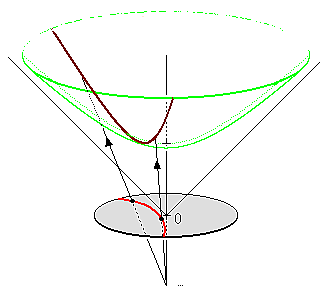
\includegraphics[height=3.5cm]{HyperboloidProjection.png} 
\end{center}
\end{frame}

\begin{frame}
\frametitle{Modelli conformi}
\begin{beamerboxesrounded}{}
In funzione della mappa conforme che lega le due varietà presentate vale:\\
\[d_{\mathbb{D}^n}(a, b) = d_{\mathbb{H}^n}(\rho^{-1}(a), \rho^{-1}(b)) \quad a, b \in \mathbb{D}^n.\]
\end{beamerboxesrounded}
\bigskip
Con:
\[ d_{\mathbb{D}^n}(a,b) = arccosh(1 + 2\frac{\| a - b \|^2}{(1 - \| a \|^2)(1 - \| b \|^2)}),\]
\[ d_{\mathbb{H}^n}(\rho^{-1}(a),\rho^{-1}(b)) = arccosh(- \langle \rho^{-1}(a),\rho^{-1}(b) \rangle_{n:1}).\]
\end{frame}

\begin{frame}
\frametitle{Media di Fréchet e problema del centroide}
\begin{beamerboxesrounded}{Media di Fréchet}
Dati $p$ punti in una varietà, la media di Fréchet di p punti è \alert{l’argomento che minimizza} la funzione \textbf{somma delle distanze al quadrato}.
\[f(\Theta) = \frac{1}{p}\sum_{i=1}^p d^2(\Theta, x^{(i)}).\]
\end{beamerboxesrounded}
\bigskip
Definendo la funzione $f$ su disco se esiste un valore di minimo allora esiste un valore di minimo anche per la funzione $\hat{f}$ definita su iperboloide.
\end{frame}

\begin{frame}
\frametitle{Media di Fréchet e problema del centroide}
\begin{beamerboxesrounded}{}
Essendo $f (x) = \hat{f} (\rho^{-1}(x))$ allora cercare il minimo di $f$ equivale a cercare il minimo di  $\hat{f} \circ \rho^{-1}$.
\end{beamerboxesrounded}
\bigskip
\`E possibile \alert{trasportare il problema} del calcolo della media di Fréchet definito su disco di Poincaré nella varietà iperboloide e viceversa.
\end{frame}

\begin{frame}
\frametitle{Algoritmi}
Abbiamo implementato i seguenti tre algoritmi nella versione riemanniana sia su disco che su iperboloide.\\~\
\begin{itemize}
    \item Algoritmo a \textbf{passo fisso}
    \item Algoritmo che si basa sul metodo di \textbf{Armijo}
    \item Algoritmo di \textbf{Barzilai-Borwein}: metodo \textbf{quasi Newton}
\end{itemize}
\end{frame}

\begin{frame}
\frametitle{Esperimenti}
\begin{beamerboxesrounded}{Obiettivo Sperimentale}
Capiremo se le due varietà sono equivalenti, non solo da un punto di vista geometrico ma anche da un punto di vista computazionale.
\end{beamerboxesrounded}
\bigskip
Abbiamo creato un dataset contenente varie (duecento) istanze del problema della media di Fréchet su disco di Poincaré, per ogni istanza ne abbiamo calcolato il limite.
\end{frame}

\begin{frame}
\frametitle{Esperimenti}
Abbiamo utilizzato un sottoinsieme del dataset per definire i parametri “liberi” degli algoritmi.\\~\

\begin{itemize}
    \item $\alpha$: dell’algoritmo a passo fisso
    \item $s$: per l’algoritmo di Armijo
\end{itemize}
\end{frame}

\begin{frame}
\frametitle{Esperimenti}
\begin{beamerboxesrounded}{Selezione parametri liberi}
\begin{itemize}
    \item Abbiamo applicato gli algoritmi con un parametro incrementale su ogni istanza del sotto-dataset
    \item Per ogni esecuzione abbiamo calcolato il numero di passi per la convergenza, generando per ogni istanza una sequenza ed alla fine ne abbiamo calcolato una media
    \item Abbiamo selezionato i parametri che minimizzano le sequenze medie sia per l’implementazione su disco che su iperboloide
\end{itemize}
\end{beamerboxesrounded}
\end{frame}

\begin{frame}
\frametitle{Scelta del parametro passo fisso}
\begin{figure}[ht]
    \begin{minipage}[b]{0.45\linewidth}
        \centering
        Disco di Poincaré\par\medskip
        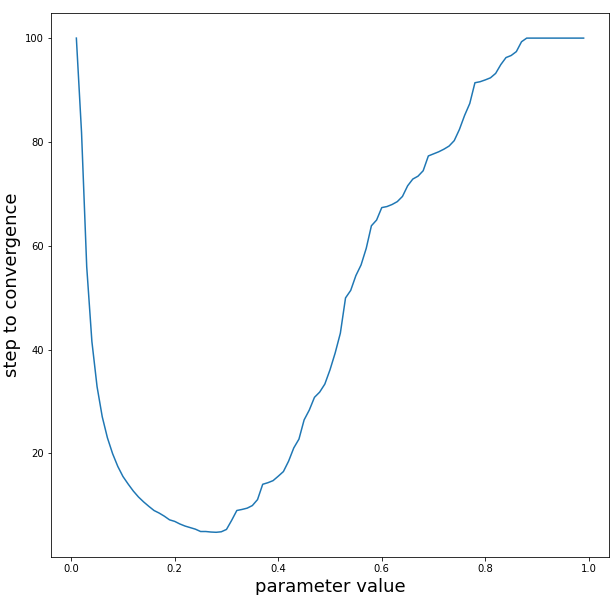
\includegraphics[width=\textwidth]{fixed_step_parameter_poincare.png}
        \caption{Punto di minimo: 0.27, valore di convergenza minimo: 7.35.}
    \end{minipage}
    \hspace{0.5cm}
    \begin{minipage}[b]{0.45\linewidth}
        \centering
        Iperboloide\par\medskip
        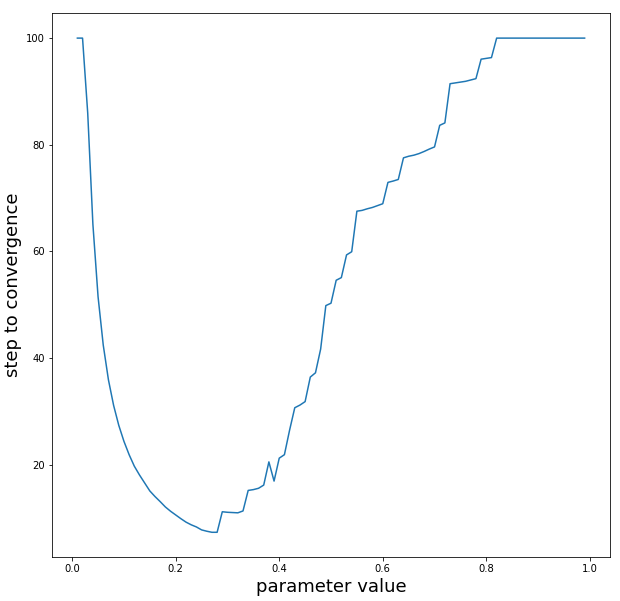
\includegraphics[width=\textwidth]{fixed_step_parameter_hyperboloid.png}
        \caption{Punto di minimo: 0.27, valore di convergenza minimo: 7.35.}
    \end{minipage}
\end{figure}
\end{frame}

\begin{frame}
\frametitle{Scelta del parametro metodo di Armijo}
\begin{figure}[ht]
    \begin{minipage}[b]{0.45\linewidth}
        \centering
        Disco di Poincaré\par\medskip
        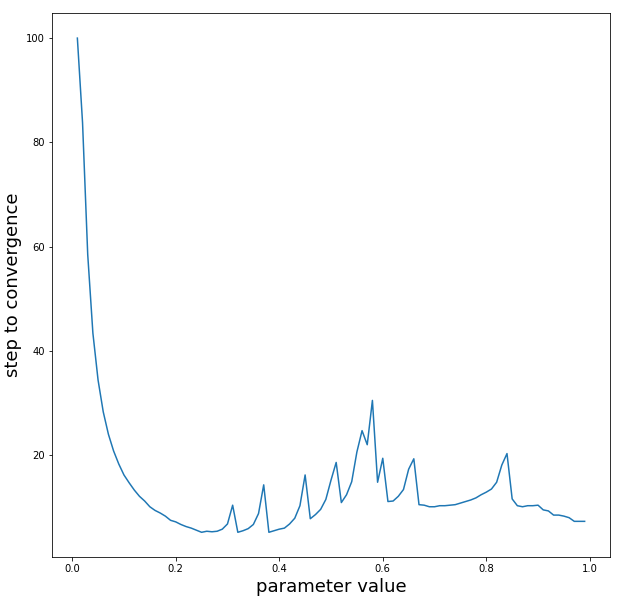
\includegraphics[width=\textwidth]{armijo_parameter_poincare.png}
        \caption{Punto di minimo: 0.26, valore di convergenza minimo: 7.9.}
    \end{minipage}
    \hspace{0.5cm}
    \begin{minipage}[b]{0.45\linewidth}
        \centering
        Iperboloide\par\medskip
        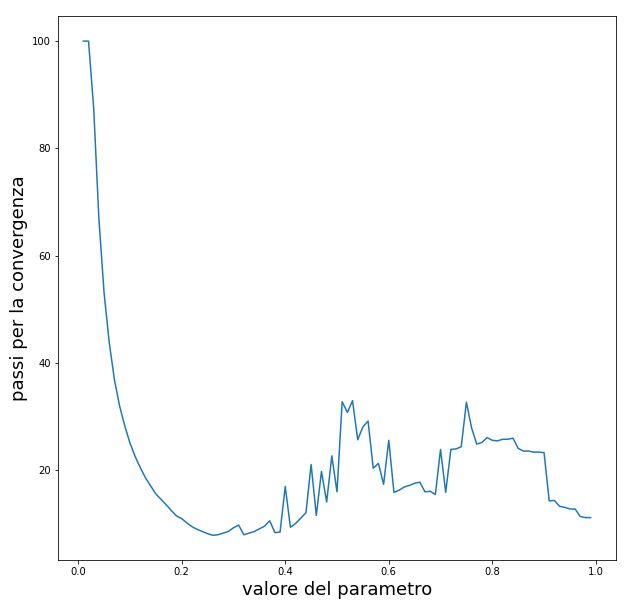
\includegraphics[width=\textwidth]{armijo_parameter_hyperboloid.png}
        \caption{Punto di minimo: 0.26, valore di convergenza minimo: 7.9.}
    \end{minipage}
\end{figure}
\end{frame}

\begin{frame}
\frametitle{Esperimenti}
\begin{beamerboxesrounded}{Metodi di confronto tra le due implementazioni}
Per ogni algoritmo lo abbiamo eseguito su ogni istanza del dataset totale creando una serie di punti $(a, b) \in \mathbb{R}^2$.\\
\begin{itemize}
    \item $a$: numero di passi per la convergenza su disco
    \item $b$: il numero di passi per la convergenza su iperboloide
\end{itemize}
\bigskip
Dalla nuvola di punti si sono eliminati quei punti con una molteplicità bassa.\\\\
Si sono calcolate due rette di regressione, la prima tramite il metodo dei \alert{minimi quadrati}, la seconda tramite l’algoritmo di \alert{Huber}.
\end{beamerboxesrounded}
\end{frame}

\begin{frame}
\frametitle{Esperimenti}
\begin{figure}[H]
    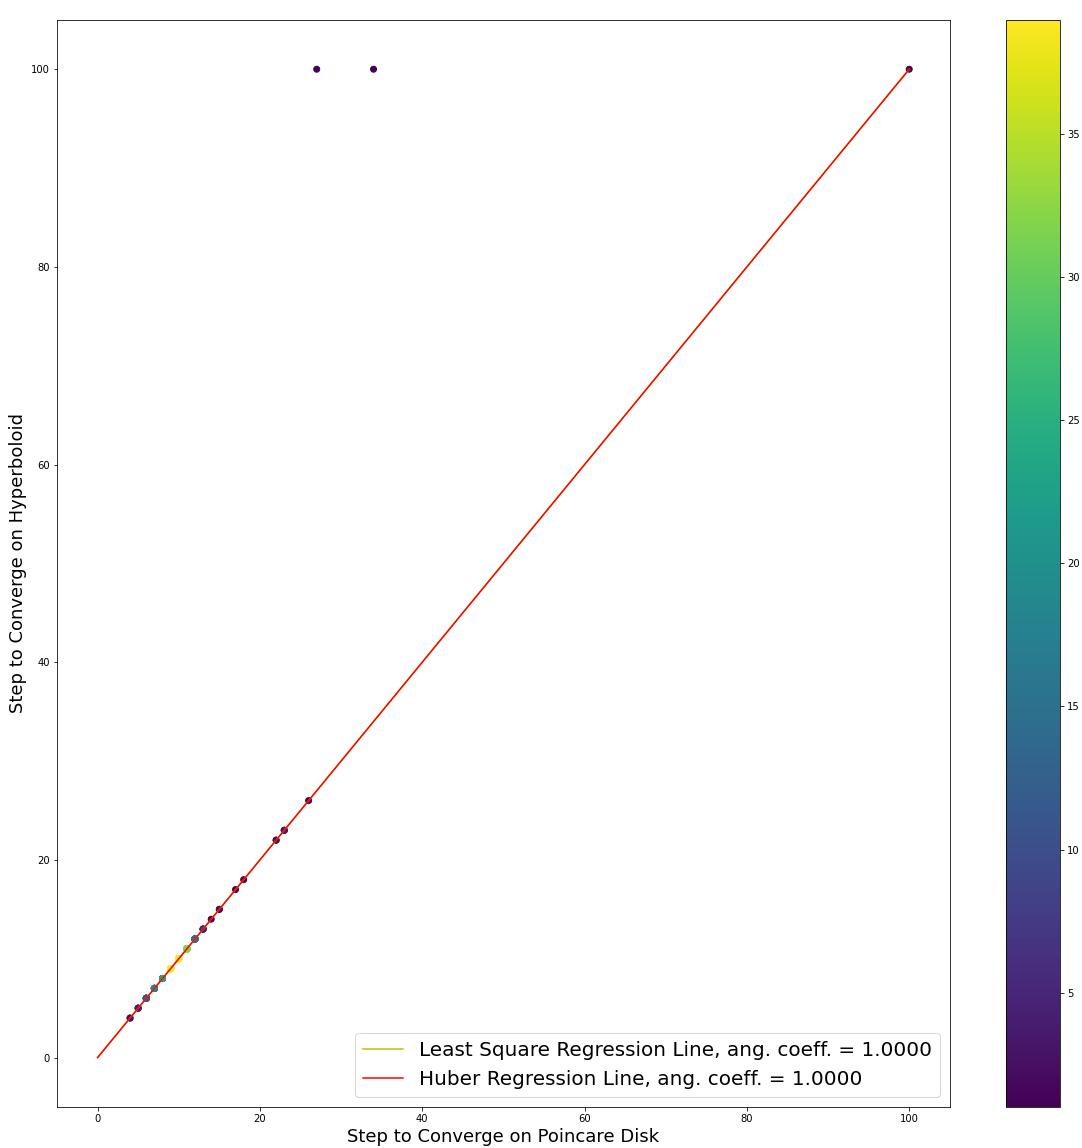
\includegraphics[height=7cm]{fixed_step_size.png}
    \caption{Nuvola di punti relativa all’algoritmo a passo fisso.}
\end{figure}
\end{frame}

\begin{frame}
\frametitle{Esperimenti}
\begin{figure}[H]
    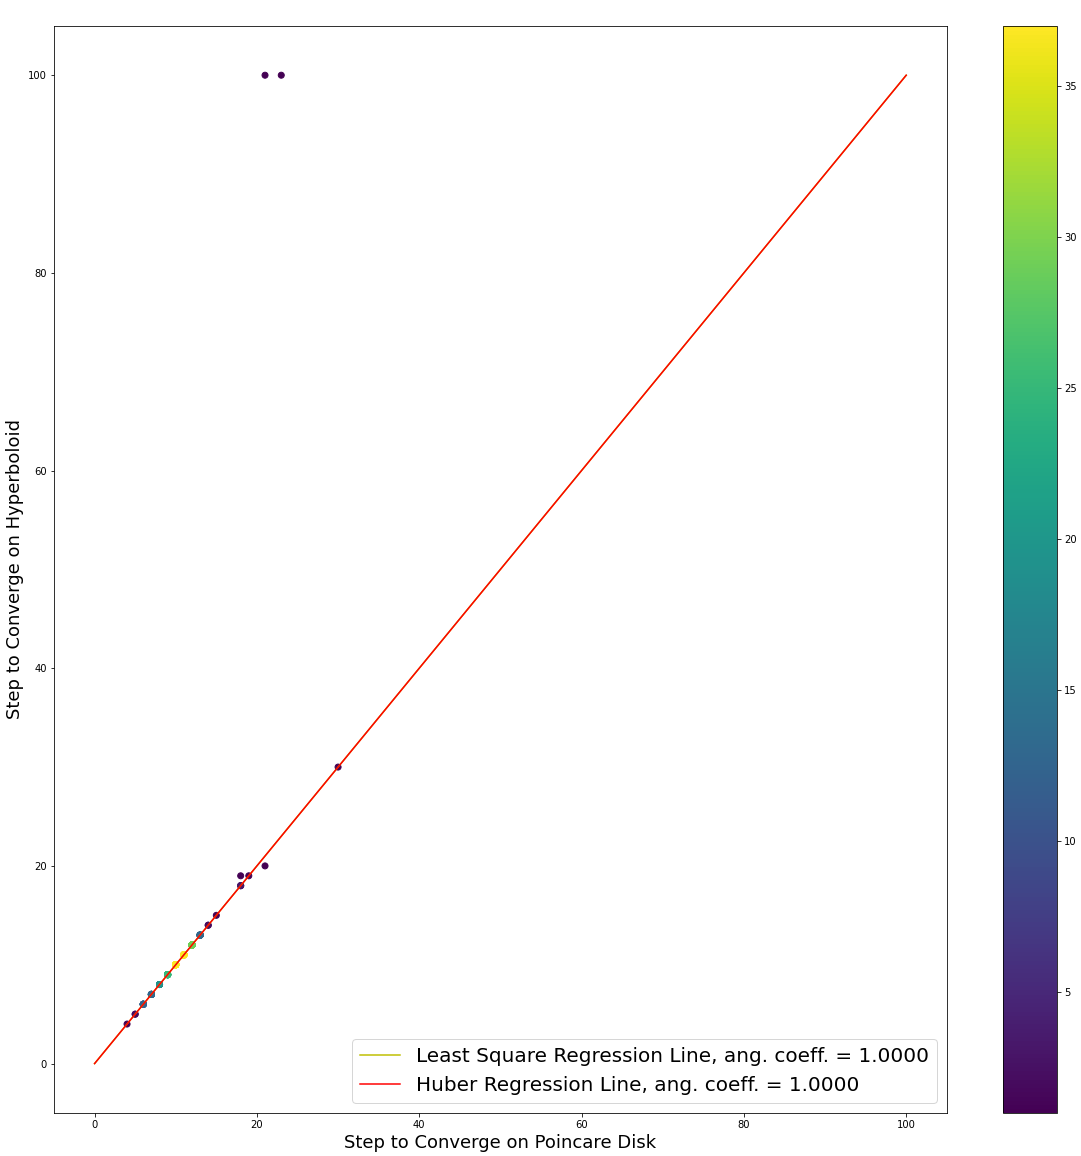
\includegraphics[height=7cm]{armijo.png}
    \caption{Nuvola di punti relativa all’algoritmo di Armijo.}
\end{figure}
\end{frame}

\begin{frame}
\frametitle{Esperimenti}
\begin{figure}[H]
    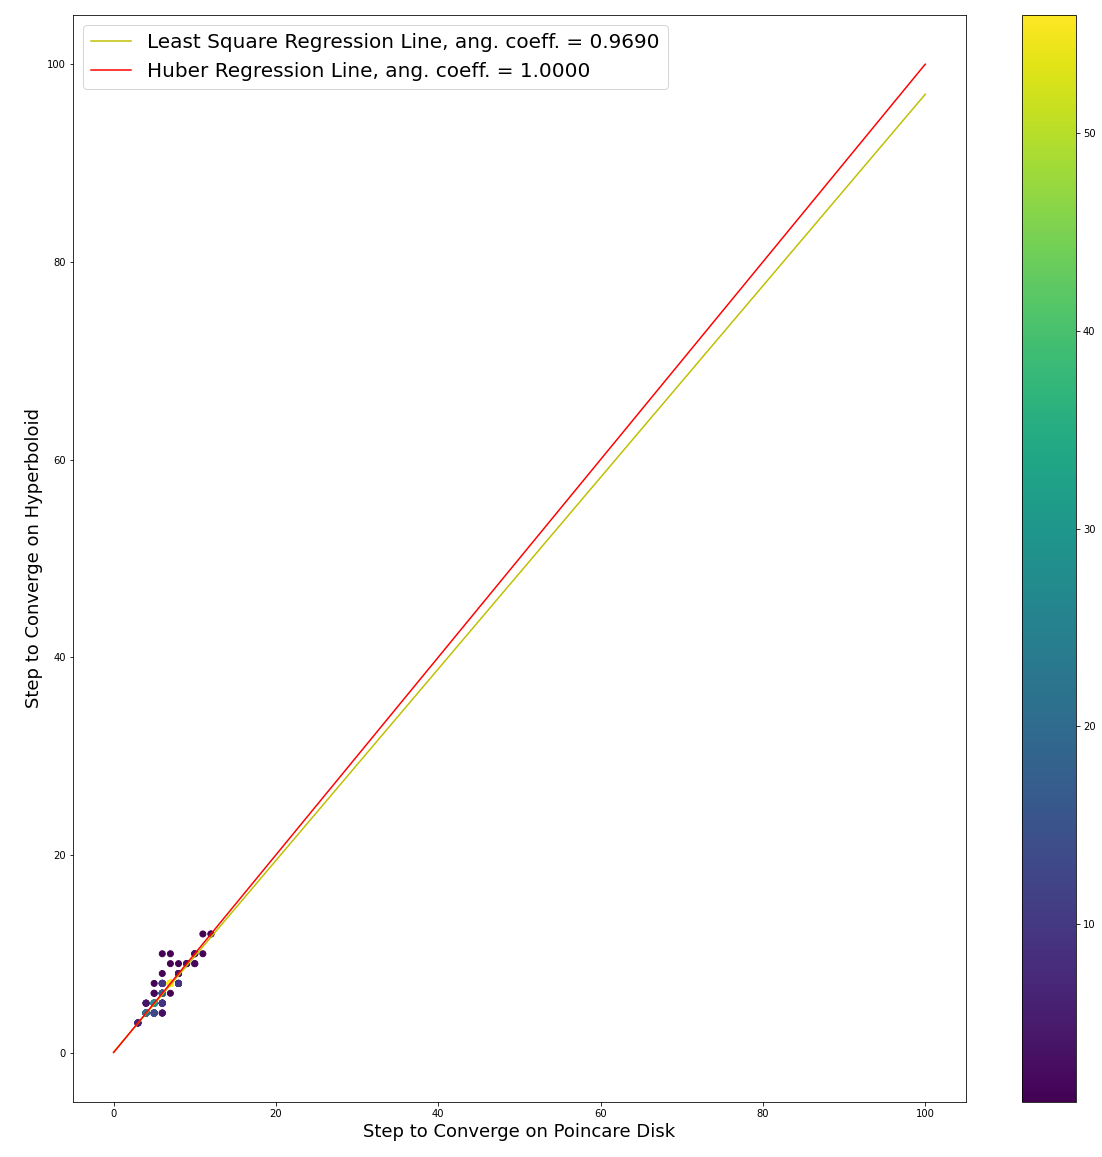
\includegraphics[height=7cm]{barzilai_borwein.png}
    \caption{Nuvola di punti relativa all’algoritmo di Barzilai-Borwein.}
\end{figure}
\end{frame}

\begin{frame}
\frametitle{Esperimenti}
\begin{beamerboxesrounded}{Convergenza media}
Confronto passi di convergenza medi per gli algoritmi implementati.\\~\
\begin{center}
\begin{tabular}{l*{6}{c}r}
                    & Passo fisso & Armijo & B.B. \\
\hline
Disco di Poincaré   & 10.5 & 10.4 & 6.13 \\
Iperboloide         & 11.2 & 11.2 & 6.8 \\
\end{tabular}
\end{center}
\end{beamerboxesrounded}
\end{frame}

\begin{frame}
\frametitle{Conclusioni}
\begin{beamerboxesrounded}{Risultato}
\`E possibile notare come l’algoritmo di \alert{Barzilai-Borwein si comporta meglio} rispetto agli algoritmi a passo fisso e di ricerca lineare (Armijo).
\end{beamerboxesrounded}
\bigskip
\begin{beamerboxesrounded}{Congettura}
\`E possibile trasferire un problema tra due varietà  conformi, deve comunque essere preservata l’esistenza di una soluzione ottima per la funzione costo.
\end{beamerboxesrounded}
\end{frame}

\begin{frame}
\frametitle{Conclusioni}
\begin{beamerboxesrounded}{Contributi}
Si sono implementate le classi per la gestione del disco di Poincaré e dell'iperboloide, che saranno proposte come aggiunta alla libreria \alert{PyManopt} implementazione python della libreria \alert{Manopt} 
\end{beamerboxesrounded}
\end{frame}

\begin{frame}
\begin{center}
Grazie per l'attenzione.
\end{center}
\end{frame}
\end{document}